\subsection{Multi-teacher and staged OPD}

Multi-Teacher On-Policy Distillation (MOPD) merges several specialized policies into one
student. Nemotron 3 Ultra routes each task family to its corresponding expert teacher and
uses the RLVR student itself as the general teacher for uncovered areas. Its full pipeline
runs two iterations: general and agentic experts produce Ultra MOPD1; that checkpoint then
becomes the next student, trained against reused, refreshed, and new experts to produce the
final model \citep{nvidia2026nemotronultra3mopd}.

NVIDIA presents this staging as a capability-merging pipeline, not explicitly as a
policy-distance ablation. A useful interpretation is that the intermediate student also
acts as a bridge: after absorbing the first expert panel, its rollouts should overlap more
with the second panel than the original student did. This can make long-horizon teacher
feedback more actionable, but the causal claim requires an ablation against one-shot MOPD.

\clearpage
\begin{figure}[htbp]
  \centering
  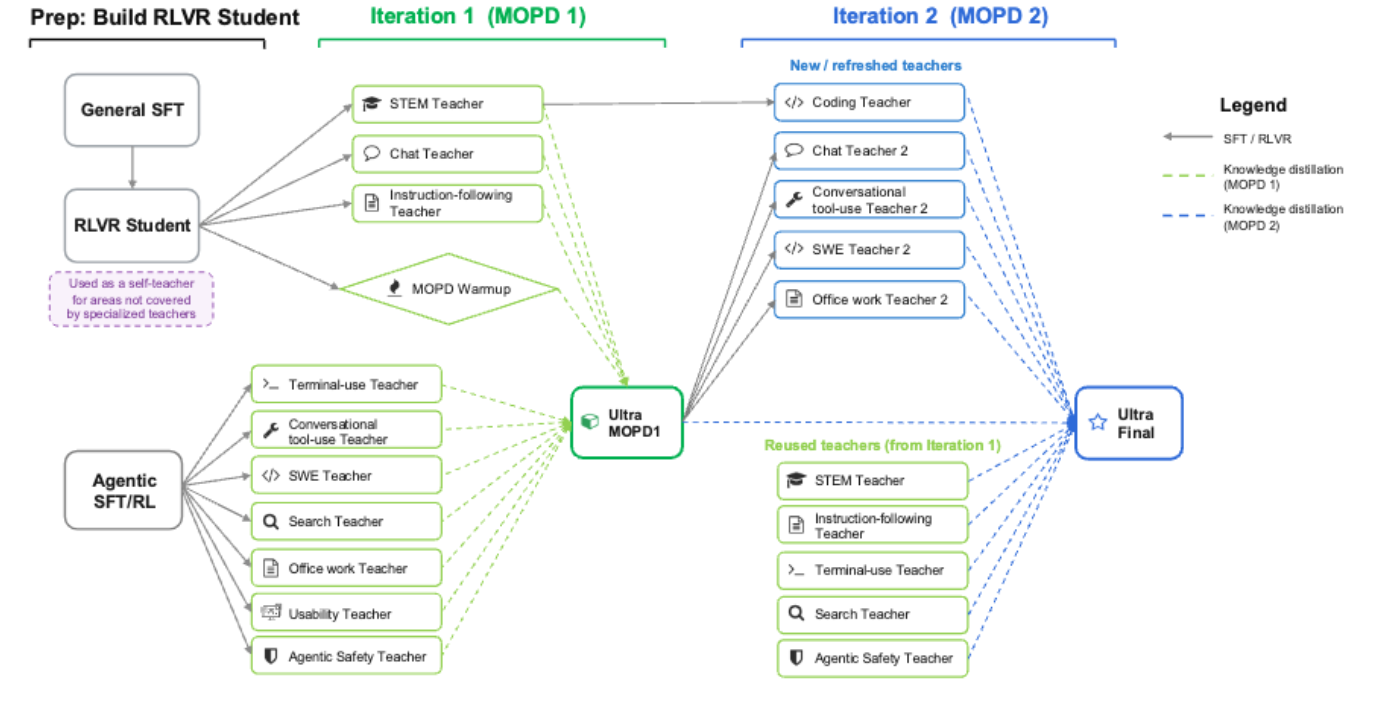
\includegraphics[width=0.98\textwidth]{figures/MOPD.png}
  \caption{Nemotron 3 Ultra's reported two-iteration MOPD pipeline. Iteration~1 merges
  general and agentic experts; Iteration~2 continues from Ultra MOPD1 with reused and
  new or refreshed teachers. Reproduced from NVIDIA's Nemotron documentation
  \citep{nvidia2026nemotronultra3mopd}.}
  \label{fig:nemotron-ultra-mopd}
\end{figure}
